%location/filename: tex/ch1.tex
%author: Anders Østevik
%Last edited: 26.05.2016
%#######--Chapter 1--#######
%Content:
%	Introduction
%	

\documentclass[main.tex]{subfiles}

%%%%%%%%%%%%%%%%%%%%%%%%%%%%%%%%%%%%%%%%%%%%%%%%%%%%%%%%%%%%%%%%%%%%%%
% LaTeX Overlay Generator - Annotated Figures v0.0.1
% Created with http://ff.cx/latex-overlay-generator/
%%%%%%%%%%%%%%%%%%%%%%%%%%%%%%%%%%%%%%%%%%%%%%%%%%%%%%%%%%%%%%%%%%%%%%
%\annotatedFigureBoxCustom{bottom-left}{top-right}{label}{label-position}{box-color}{label-color}{border-color}{text-color}
\newcommand*\annotatedFigureBoxCustom[8]{\draw[#5,thick,rounded corners] (#1) rectangle (#2);\node at (#4) [fill=#6,thick,shape=rectangle,draw=#7,inner sep=2pt,font=\sffamily,text=#8] {\textbf{#3}};}
%\annotatedFigureBox{bottom-left}{top-right}{label}{label-position}
\newcommand*\annotatedFigureBox[4]{\annotatedFigureBoxCustom{#1}{#2}{#3}{#4}{red}{white}{red}{black}}
\newcommand*\annotatedFigureText[4]{\node[draw=none, anchor=south west, text=#2, inner sep=0, text width=#3\linewidth,font=\sffamily] at (#1){#4};}
\newenvironment {annotatedFigure}[1]{\centering\begin{tikzpicture}
    \node[anchor=south west,inner sep=0] (image) at (0,0) { #1};\begin{scope}[x={(image.south east)},y={(image.north west)}]}{\end{scope}\end{tikzpicture}}
%%%%%%%%%%%%%%%%%%%%%%%%%%%%%%%%%%%%%%%%%%%%%%%%%%%%%%%%%%%%%%%%%%%%%%

\begin{document}

\chapter{Introduction}

\section{Large Hadron Collider}

The \gls{lhc} is the largest and most powerful particle collider in the world. It was built by the \gls{cern} \cite{cernweb} between 1998 and 2008, and had its first start-up on 10 September 2008. This massive machine lies 175 metres under ground, beneath the France–Switzerland border near Geneva, Switzerland; and consists of a $27~\kilo\meter$ long circular tunnel of superconductor magnets with additional accelerating structures. Its basic operation is to accelerate particles (protons and heavy ions, e.g. Pb) in bunches\footnote{The particles are accelerated in bunches to increase the probability that a collision will occur.} to near the speed of light in opposite directions and collide them. The particle bunches are accelerated along two parallel beam lines running through the superconductor magnets, and collided at four locations were experiments like; ATLAS\cite{atlasweb}, ALICE\cite{aliceweb}, CMS\cite{cmsweb} and LHCb\cite{lhcbweb} take place. As of 20 May 2015, the \gls{lhc} can achieve beam energies up to $13~\tera e\volt$, or $6.5~\tera e\volt$ per beam. Figure \ref{fig:lhcov} shows an overall view of the \gls{lhc} experiments.

\begin{figure} % H(strictly put HERE > h!)
% h(here), !(force), t(top), b(bottom), p(on extra page)
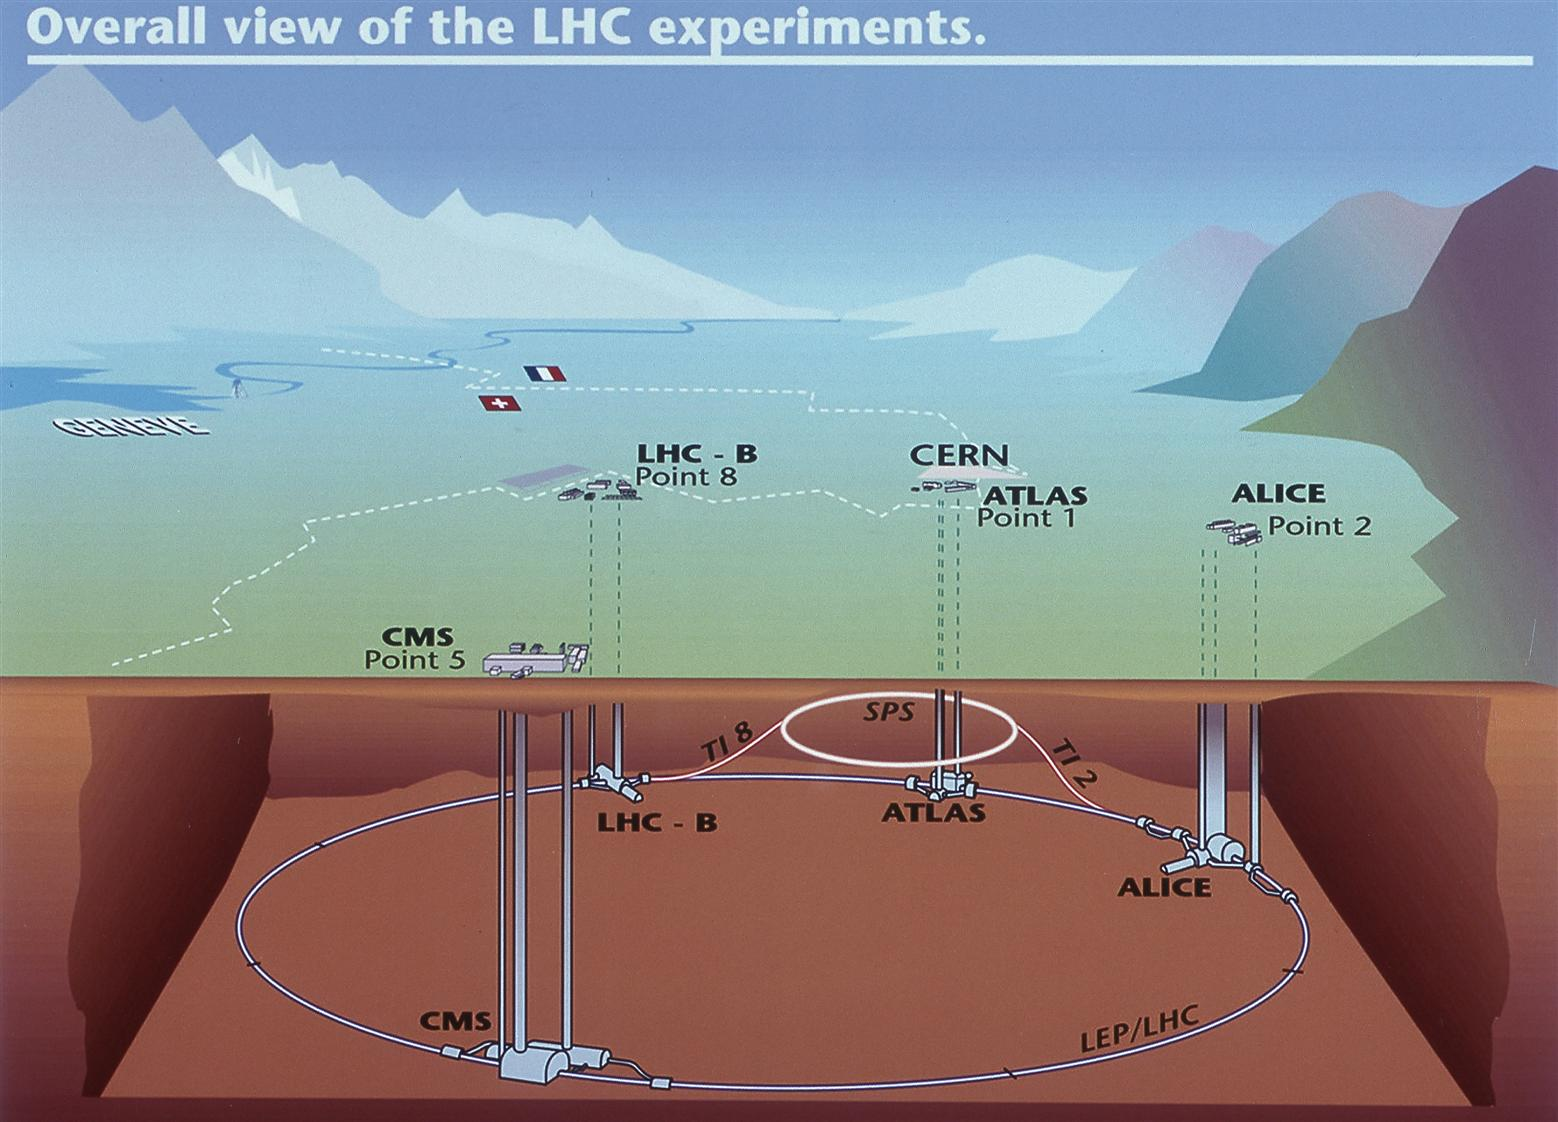
\includegraphics[width=0.7\linewidth]{../img/lhc.jpg}  \\[0.1 cm]
\caption{LHC overview \cite{lhcpic}.}
\label{fig:lhcov}
\end{figure}

\section{High-Luminosity LHC}

The future upgrade of the \sebo{\gls{lhc}} accelerator, the \gls{slhc}, has its goal of increasing the beam luminosity by ten times. This will lead to a corresponding growth of the amount of data to be treated by the data acquisition systems, and an increase in radiation. This will thus require high rate data links and \glspl{asic} capable of tolerating high doses of radiation.

To address these needs, the \gls{gbt} \glspl{asic} and transmission protocol was developed to provide a high radiation tolerant, high speed, optical transmission line capable of simultaneous transfer of readout data, timing and trigger signals in addition to slow control and monitoring data.

\section{The Gigabit Transceiver system}
As illustrated in figure \ref{fig:gbtsys}, the \gls{gbt} system can be separated into two parts: The on-detector part, and the off-detector part of the system. The below sections gives a brief description of these:

\begin{figure}[!b] % H(strictly put HERE > h!)
% h(here), !(force), t(top), b(bottom), p(on extra page)
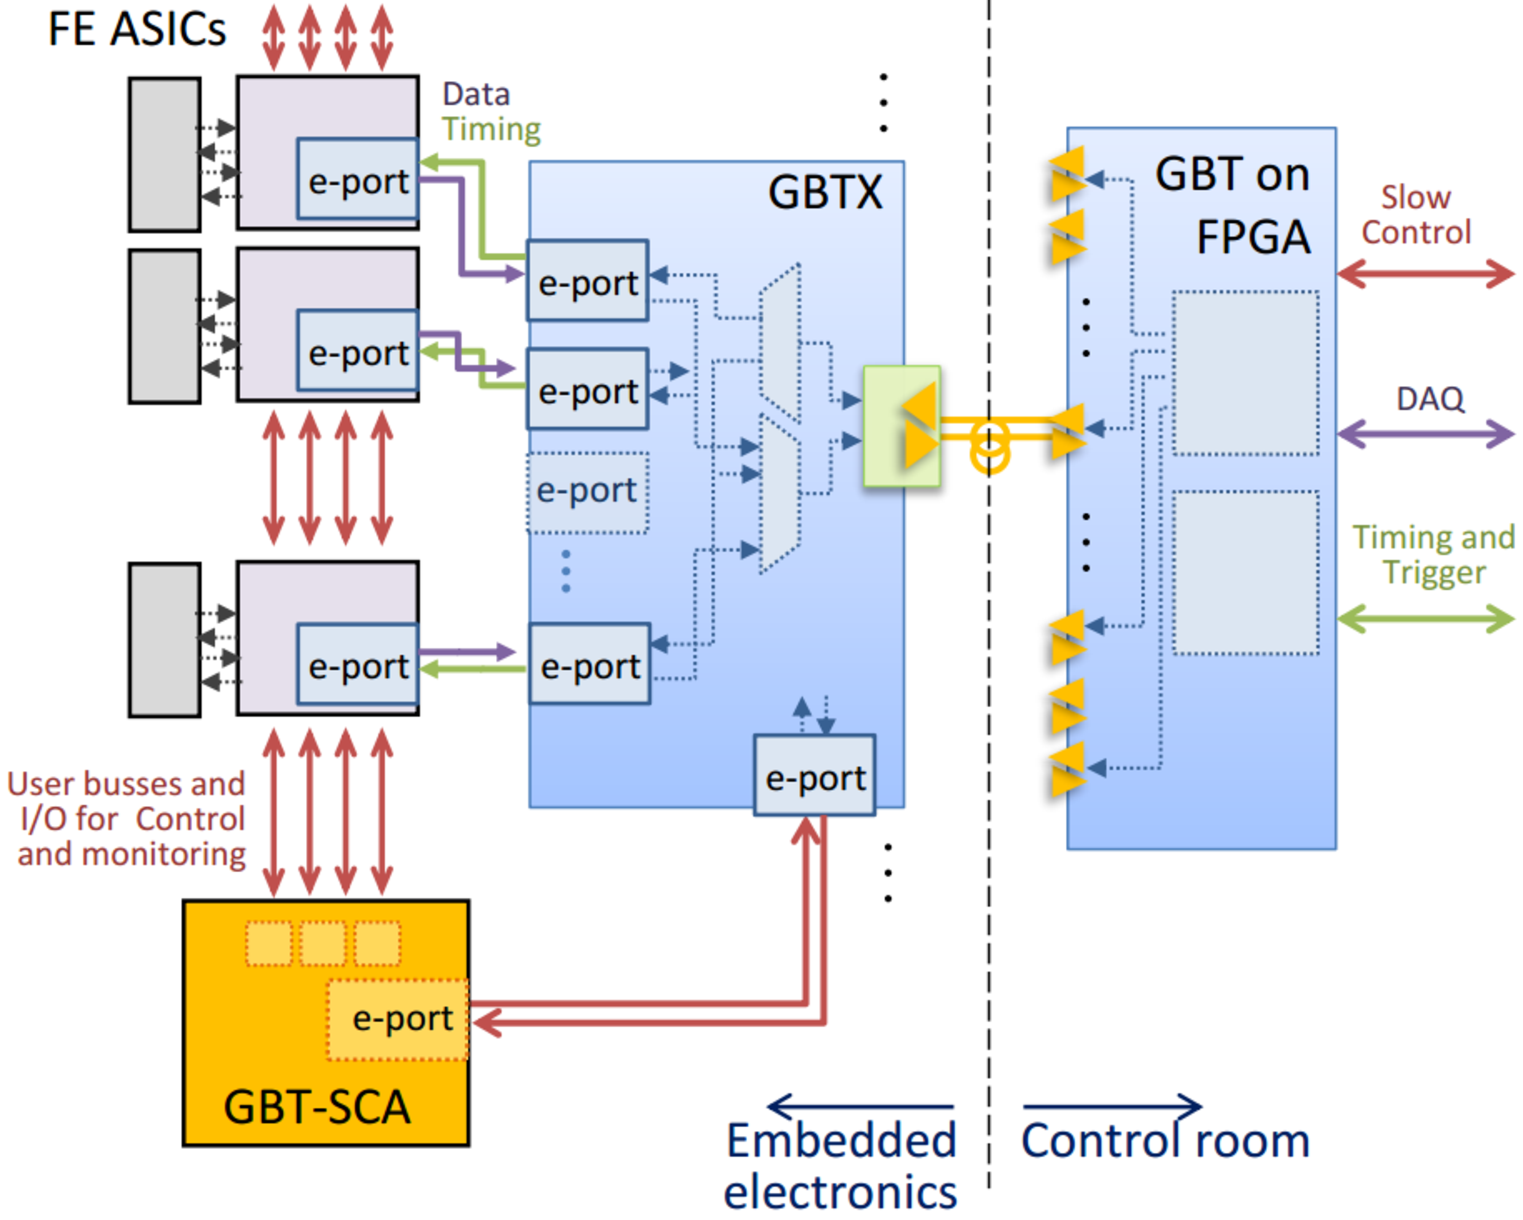
\includegraphics[width=0.7\linewidth]{../img/gbtsys}  \\[0.1 cm]
\caption{The GBT-link in its entirety. The on-detector (Embedded electronics) consists of custom made \glspl{asic} with an optical link connecting the off-detector (control room) \gls{fpga} with the GBT-FPGA implemented. \cite[Figure 1]{gbtscapres14}.}
\label{fig:gbtsys}
\end{figure}

\subsection{On-detector}
The on-detector part consists of radiation hard GBT \acrshort{asic}s that will provide interface and data transmission to the detectors and will thus be located in the radiation zone. These \glspl{asic} are used to implement bi-directional multipurpose $4.8~\giga\bit\per\second$ optical links for the high-energy physics experiments.

\subsubsection{GBTx}
The GBTx \gls{asic} is a serializer-de-serializer chip responsible for the high speed bi-directional optical link. It has a bandwidth of $3.2 - 4.8~\giga\bit\per\second$, and combines three data paths for Trigger and Timing Control (TTC), Data Acquisition (DAQ) and Slow Control (SC) information in one physical link; using two optical fibers. The GBTx encodes and decodes this information into what is known as the GBT-Frame, and provides interface to the front end electronics embedded in the detectors. \cite{gbtxman11}

\subsubsection{GBT frame formats} \label{sub:encodings}
 The GBTx transmits a 120-bit frame every $25~\nano\second$ ($40~\mega\hertz$), which is triggered by LHC particle bunch crossings. The GBTx supports three different encoding modes: "GBT-Frame", "8B/10B" and "Wide-Bus" mode. Figure \ref{fig:gbtframe} illustrates the "GBT-Frame" mode. The frame is divided into four parts: Header (H), Slow Control (SC), User Data (D) and Forward Error Correction (FEC). The Header field is a 4-bit field transmitted at the beginning of each frame, used to synchronize the data stream at the frame level. The header field can be set to "idle" (0110) or "data" (0101). The Slow Control field is a 4-bit field dedicated for routine and control operations that do not require precise timing. The User Data field is a 80-bit field reserved for generic transmission of data with a corresponding bandwidth of $3.2~\giga\bit\per\second$. The remaining field reserves 32 bits for Forward Error Correction. This involves using Reed-Solomon encoding capable of correcting up to 16 concecutive corrupted bits. To achieve DC-balancing, a self-synchronizing scrambler distributes the 0's and 1's in the data stream.

The "8B/10B" and "Wide-Bus" mode share simularities with the "GBT-Frame" mode, but favors data width over reduced error correction (the "Wide-Bus" has none). Both modes are only available in the transmitter part of the GBTx, but requires less resources from the \gls{fpga} (\ref{sec:offdetect}) than the "GBT-Frame". The "8B/10B" does not require scrambling because it is in itself DC-balanced \cite{gbtxman11}. These two modes are not yet available in the GBT FPGA example design. Both GBTx encoding and decoding operations can be done within a single clock cycle at $40~\mega\hertz$. 
 
\begin{figure} % H(strictly put HERE > h!)
% h(here), !(force), t(top), b(bottom), p(on extra page)
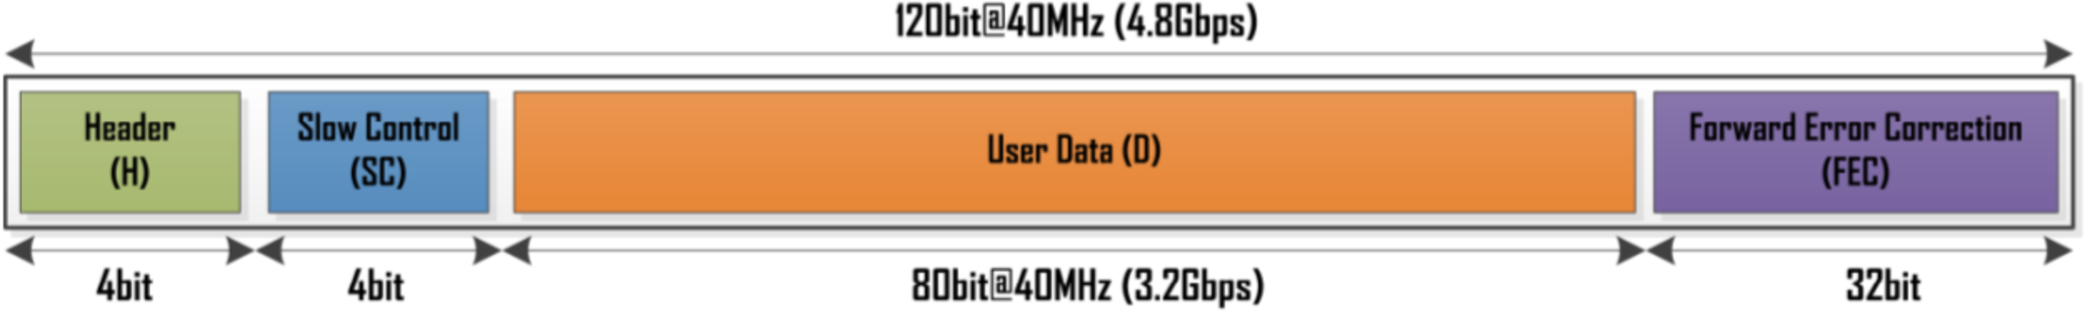
\includegraphics[width=\linewidth]{../img/gbtframe}  \\[0.1 cm]
\caption{The GBT-Frame format. \cite[Figure 4]{gbt_fpga}.}
\label{fig:gbtframe}
\end{figure}

\subsubsection{GBT-SCA}

The \gls{sca} \gls{asic} is the part of the \gls{gbt} chipset which distributes control and monitoring signals to the front-end electronics embedded in the detectors. It connects to the GBTx through a dedicated $80~\mega\bit\per\second$ e-link (\ref{sec:elinks}) and provides a number of user interface options for the front-end detectors, which includes: SPI, \acrshort{iic}, JTAG and a number of \acrshort{gpio}s \cite{gbtsca15}. \\

\noindent
All chips have been implemented using a commercial $130~\nano\meter$ process because of benefits regarding inherent resistance to ionising radiation \cite{gbtpro10}.

\subsection{Off-detector} \label{sec:offdetect}
The off-detector part is located in the counting room and consists of a \gls{cru}, that will provide an interface between the detector \acrshort{asic}s and an online computer farm, with the GBTx as the middle joint. The \gls{cru} consists of \gls{cots} components, mainly an \gls{fpga}, and will through optical links receive the data from the radiation detector.

\subsubsection{FPGA - Cyclone V GT} \label{sec:cyclone}

Altera's Cyclone V GT \gls{fpga} board was chosen for use in this thesis. It was chosen mainly because of the on-board transceivers that are capable of reaching speeds that surpass the requirements of the \gls{gbt}-\gls{fpga} \gls{mgt}, i.e $4.8~\giga\bit\per\second$; "GT" indicates that the \gls{fpga} has transceivers that support speeds up to $6~\giga\bit\per\second$ \cite{altera_cvoverview15}.

Originally, a Terasic Cyclone V SX development board was aquired for use with this thesis. The Terasic board has advantages over the Cyclone V GT board in terms of communication with the outside world, such as an on-board Usb-to-Uart interface (more on this  in chapter \ref{chap:sercom}). However, it was discovered that the transceivers on the Terasic board were not fast enough for the \gls{gbt} \gls{mgt}; maximum supported transceiver speed is only $3.125~\giga\bit\per\second$ \cite{altera_cvoverview15}. Because of this, the more powerful Cyclone V GT \gls{fpga} development board was ordered, replacing the Terasic.

\subsubsection{GBT-FPGA project}

The GBT-FPGA project provides a firmware library for Altera and XilinX \glspl{fpga} for communication with the GBTx chipset. It allows for one or several GBT links of type "Standard" or "Latency-Optimized" (The latter providing low, fixed and deterministic latency). Each GBT link is composed of three components: a GBT Rx, a GBT Tx and an \gls{mgt}. The GBT Rx is responsible for receiving, decoding and de-scrambling the data from the \gls{mgt}.  The GBT Tx is responsible for scrambling and encoding data before transmitting it through the \gls{mgt}. The \gls{mgt} is responsible for the actual transmitting, receiving, serialization and de-serialization of the \gls{gbt} data. It is divided into a transmitter and a receiver: The transmitter shifts in $40~\bit$ words from the GBT Tx, serializes the data and sends it out with the help of a dedicated \acrshort{pll} that generates a serial clock of $2400 \mega\hertz$. The receiver de-serializes the incoming data before shifting it to the GBT Rx. The receiver contains a \gls{cdr} block to recover the clock signal directly from the incoming data stream \footnote{To be able to recover the clock using a \gls{cdr}, it is important that the serial data has even transitions of 1's and 0's. This is one of the reasons why scrambling the data is important.}. The \gls{mgt} requires an external clock of $120~\mega\hertz$ \cite{gbt_fpga}.\\
The GBT link supports all three encodings described in section \ref{sub:encodings}. 

\subsubsection{GBT-example design}
The firmware library comes with an example design that incorporates a single GBT link of the "Standard" type. Included in the example is a pattern generator, connected to the GBT Tx; a pattern checker, connected to the GBT Rx; and a user control interface implemented using the Quartus-bound \gls{issp}. The example enables for external and internal loopback testing.

\section{Versatile Link Demo Board} \label{sec:vldb}

The \gls{vldb}, shown in figure \ref{fig:vldb}, is the evaluation kit for the radiation hard optical link. It includes the main elements of the GBT Link, the radiation hard \glspl{asic}; GBTx, GBT-SCA and VTRx/VTTx (optical-link modules), in addition to radiation hard DC/DC converters. The \gls{vldb} has 20 e-links reachable through \acrshort{hdmi}-connectors that connects to the front-end electronics, and a fiber-optical link that connects to the off-detector \gls{fpga}.\\

\begin{figure}[!b]
        \begin{annotatedFigure}
            {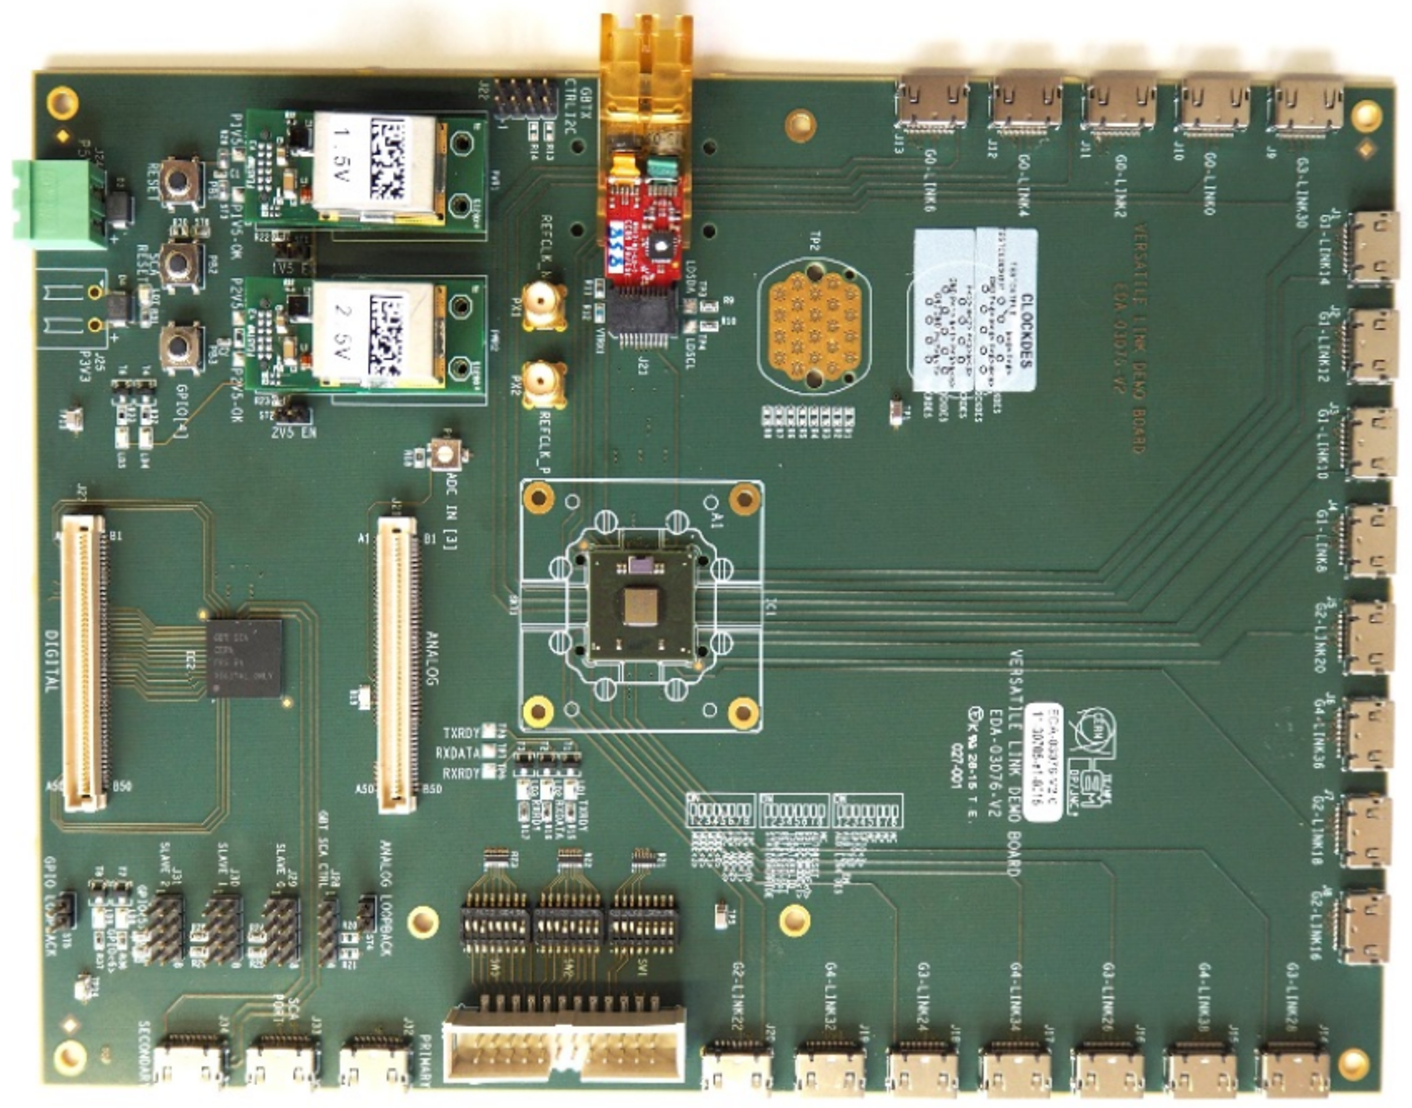
\includegraphics[width=0.6\linewidth]{../img/vldb}}
            \annotatedFigureBox{0.18,0.6}{0.35,0.92}{Dc/Dc Converters}{0.1,0.55}%bl
            \annotatedFigureBox{0.122,0.35}{0.23,0.47}{GBT-SCA}{0.1,0.3}%tr
            \annotatedFigureBox{0.42,0.65}{0.5,1.0}{VTRx/VTTx}{0.65,0.77}%bl
            \annotatedFigureBox{0.37,0.35}{0.54,0.55}{GBTx}{0.55,0.3}%tr
        \end{annotatedFigure}
\caption{Versatile Link Demo Board overview \cite{vldbposter}.}
\label{fig:vldb}
\end{figure}

\section{E-Links} \label{sec:elinks}
E-links are electrical local duplex  serial links suitable for transmission over PCBs or cables, within a distance of a few meters, and can operate at any data rate up to $320~\mega\bit\per\second$ \footnote{The GBTx can only handle $320/160/80~\mega\bit\per\second$}. It was designed with the GBTx in mind, having radiation hard and single event upset (SEU) resistant transmitter and receiver blocks. The e-links supports both \acrshort{slvs} and \acrshort{lvds} electrical standards \cite{elinks}. Each E-link consists of three differential signal lines: a clock line (dClk+/dClk-), a downlink output (dOut+/dOut-) and a uplink input (dIn+/dIn-).

The GBTx arranges e-links in 5 groups, with up to 8 e-links per group corresponding to 16 bits in the uplink and the downlink frames; making a total of 80 bits \cite{gbtxman11}. Each group can be programmed to data rates of $80~\mega\bit\per\second$, with 8 e-links per group; $160~\mega\bit\per\second$, with 4 e-links per group; or $320~\mega\bit\per\second$, with 2 e-links per group. Faster data rates comes with the expense of less physical e-link connections available for the front-end detectors.

\section{Primary objective}
The primary objective of this thesis has been to design a \gls{cru} control interface software, along with the design of a \gls{pcb} that provides physical connection between the \gls{cru} (FPGA) and the \gls{vldb} card. The control interface was developed with the goal of one day replacing the Quartus-bound \gls{issp}, which is used today to manipulate the \gls{gbt} control-signals; and instead introduce a cross-platform, open-source solution. The software is not completed, but well on its way to become usable. The \gls{pcb} is completed, but some testing remains along with a full system test with the GBTx involved.

\section{Outline}
This thesis is devided into six chapters, including this one. Chapter \ref{chap:cycv} gives a brief description of the transceiver technologies that enables communication between the GBTx and the CRU. Chapter \ref{chap:pcb} gives a brief overview over the process of designing a PCB that connects the \gls{fpga} and the \gls{vldb} togheter using e-links and optical link. Chapter \ref{chap:sercom} gives a brief overview of the development of the PC to CRU software design, both on the software and hardware side. Chapter \ref{chap:tests} presents the different tests performed on the developed PCB, software and hardware. Finally, chapter \ref{chap:conc} summarizes and concludes the thesis.

%\todo{General:\\PLLs\\CPRI?\\}

\chapter{Cyclone V Transceiver Technology} \label{chap:cycv}

For the \gls{fpga} to be able to transmit and receive serial data in the gigahertz domain, a high-speed transceiver is required. The Cyclone V GT-series supports a number of transceiver technologies through the \gls{hsmc} physical interface that can reach speeds up to $5.0\ \giga\bit\per\second$. This section gives a general description of some of these protocols.

\section{Differential Signals} \label{subsec:diffsig}

Common for all protocols described here is the fact that the signals are treated differentially. While a single ended signal involves one conductor between the transmitter and receiver, with the signal swinging from a given voltage to ground; differential signals involve a conductor pair of two signals that are identical, but with opposite polarity. The pair would ideally have equal path lenghts in order to have zero return currents, avoiding problems like \gls{emi}. In addition, placing the signals as close as possible to one another will give benefits in terms of common-mode noise rejection \cite{douglas01}.\\

When implemented correctly, differential signals have advantages over single ended signals such as effective isolation from power systems, minimized crosstalk and noise immunity through common-mode noise rejection. It also improves S/N ratio and effectively doubles the signal level at the output $(+v - (-v) = 2v)$, which makes it especially useful in low level signal applications. The disadvantage comes in an increase in pin count and space required, since differential signals consists of two wires instead of one \cite{douglas01}.

\section{Low-Voltage Differential Signaling} \label{sec:lvds}

\gls{lvds} is said to be the most commonly used differential interface. The interface offers a low power consumption with a voltage swing of $350\ \milli\volt$ and good noise immunity. With the right conditions, the standard can be able to deliver data rates up to $3.125\ \giga\bit\per\second$ \cite{ti08lvds}.\\

The Cyclone V GT board has 17 \gls{lvds} channels available on the \gls{hsmc} port A connector. The channels have the ability to transmit and receive data at a rate up to $840\ \mega\bit\per\second$, with support for serialization and de-serialization through internal logic \cite{altera_cvoverview15}.

\section{Current-Mode Logic}

For data rates that exceeds $3.125\ \giga\bit\per\second$, \gls{cml} signaling is preferred. This is due to the fact that certain communication standards such as \acrshort{pci}-express, \acrshort{sata} and \acrshort{hdmi}, shares consistency with CML in signal amplitude and reference to $Vcc$. CML can reach a data rate in excess of $10\ \giga\bit\per\second$, but has a higher power consumption than \gls{lvds}, with a voltage swing of approximately $800\ \milli\volt$ \cite{ti08lvds}.\\

The Cyclone V GT board has 4 Pseudo-\gls{cml} (PCML) channels available on both port A and B \gls{hsmc} connectors. The channels have the ability to transmit and receive data at a rate up to $5.0\ \giga\bit\per\second$, just over the $4.8\ \giga\bit\per\second$ range required by the \gls{gbt} \gls{mgt} \cite{altera_cyclonekit}.


%\subsection{CPRI}

%\subsection{Phase-Locked Loops}

%A \gls{pll} is a device

%\gls{cpri}


%\begin{align}
%	 b_1 &= s_{11}a_1 + s_{12}a_2 \\
%	 s_{21}a_1 + s_{22}a_2 &= b_2
%\end{align}


\end{document}

